\section{GPaaScaler architecture}

This section presents our auto-scaler architecture named \emph{GPaaScaler}, which continuously listens the instances of events \emph{e.g.,} response time, green energy availability, working modes of application etc., pushed by SaaS and IaaS in a changing environment. Furthermore, it inherits the capability to actuate both at application and at infrastructure level.
We use the most popular self-adaptive design framework: Monitor-Analyze-Plan-
Execute-Knowledge (MAPE-K) loop \cite{vision} for our auto-scaler.
Our contribution lies on the \emph{analyze} and \emph{plan} (A-P) block of this autonomic framework.

\begin{figure} [ht]
\centering
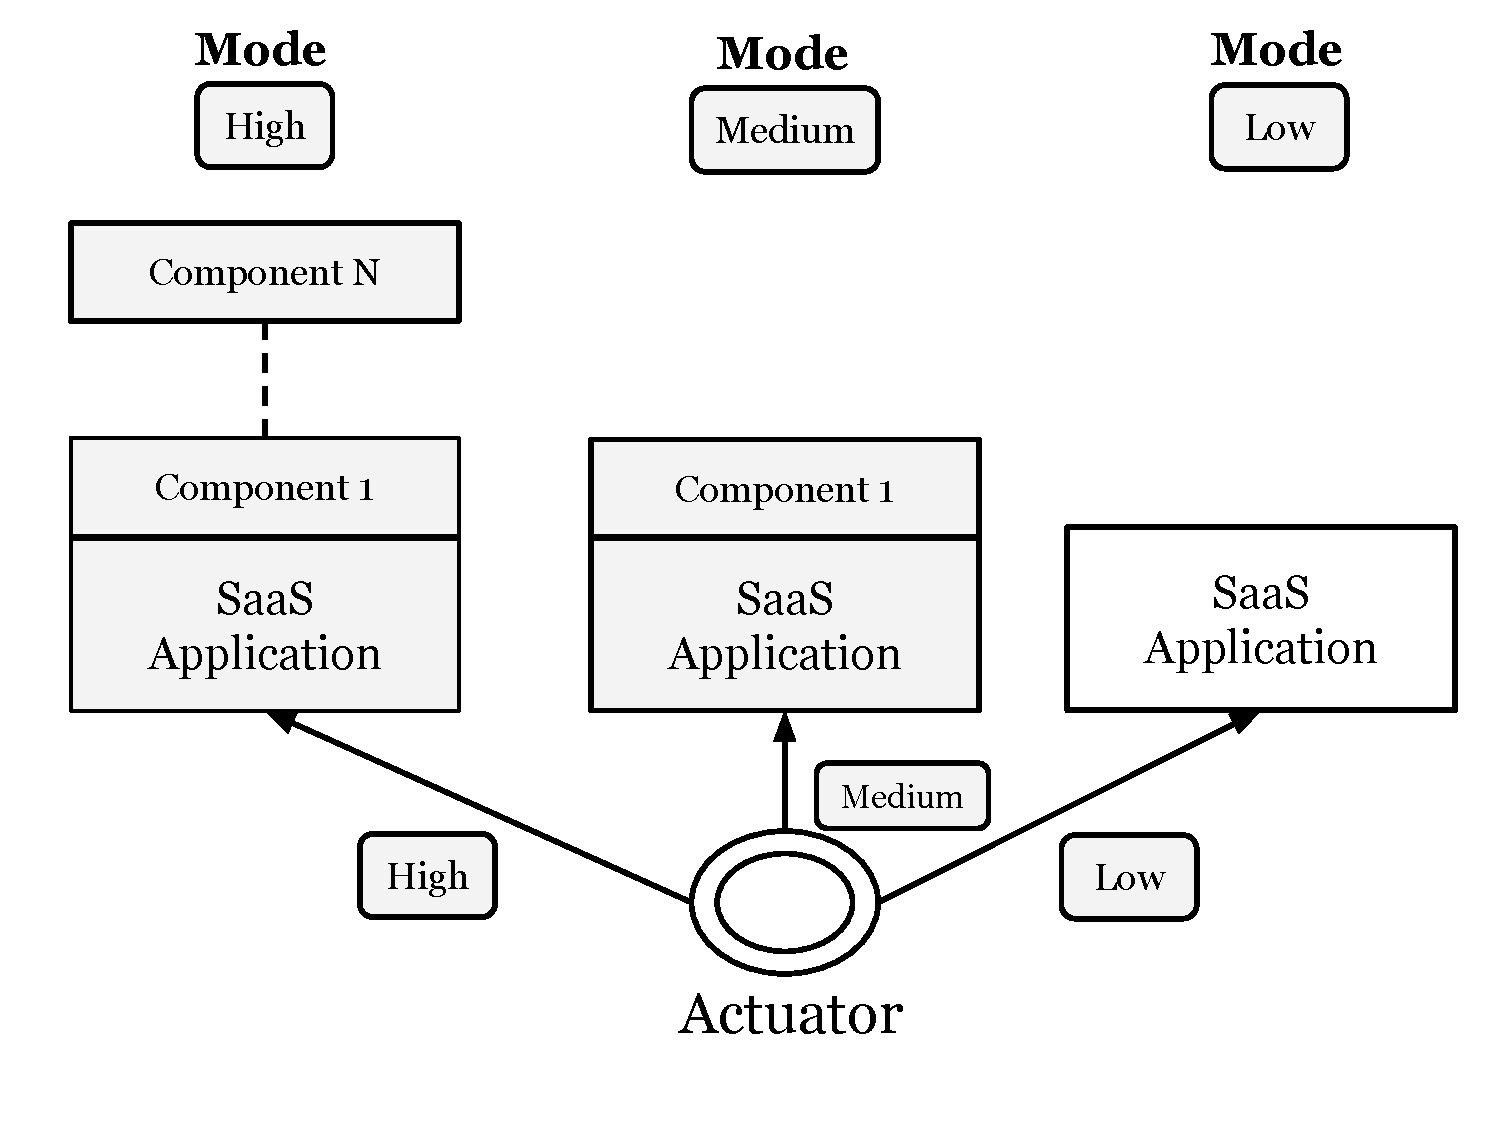
\includegraphics[scale=.32]{Graphs/action_1.pdf}
\caption{Applications mode under different service level}
\label{fig:modes}
\end{figure}

Monitoring (M) block pushes listened events to \emph{Analyze} block from SaaS layer (\emph{i.e.,} response time, workload, application's working mode, etc.) and IaaS layer (\emph{i.e.,} quality of energy). Analyze (A) block is responsible for analyzing and decoupling events to extract the pertinent information and feed appropriate event to the event handler at the SaaS controller. Once the events are 
received, Plan (P) block analyzes and matches to the predefined reactive or proactive rules and create a
configuration plan. The Execution (E) block is consist of two types of actuator \emph{i.e.,} SaaS and IaaS.
After the configuration plan, if needed, SaaS controller triggers action through SaaS actuator.
We propose three user experience levels. Mode High refers to high user
experience while Mode Medium and Mode Low indicate to medium and low user experience respectively (see Figure \ref{fig:modes}). When current application behavior deviates from target system state in terms of objective metrics, the auto-scaler gracefully downgrades the user experience from higher mode to lower mode and vice-versa through proper actuator value. Once SaaS actuator trigger the adaptation plan, it passes request for addition/removal of resources event as «RequestEvent» to IaaS controller if the former controller decides that application needs more/less resources, which is shown at Figure \ref{fig:GPaaScaler}. Following the event, IaaS controller decides to take action via traditional infrastructure API (built in IaaS actuator) that is \emph{scale-in} and \emph{scale-out} or wait/discard the request issued by the SaaS controller. Therefore, the execution block is composed of two types of actuators, \emph{i.e.,} SaaS and IaaS actuator, which can be seen at Figure \ref{fig:GPaaScaler}. In addition, \encircle{1}, \encircle{2} and \encircle{3} depict the task flow of our auto-scaler, 
whereas, the sequential flow in an ordered way (from $1.a$ to $1.e$) is presented at the Figure \ref{fig:GPaaScaler} for highlighting the control flow of the event.
In summary, IaaS controller only gets activated if SaaS controller issues any «RequestEvent». However, our proposed IaaS controller are unware of resource allocation strategy, for instance, what types of VM is to be added/removed or in which server VM is to be located etc.  




\begin{figure} [ht]
\centering
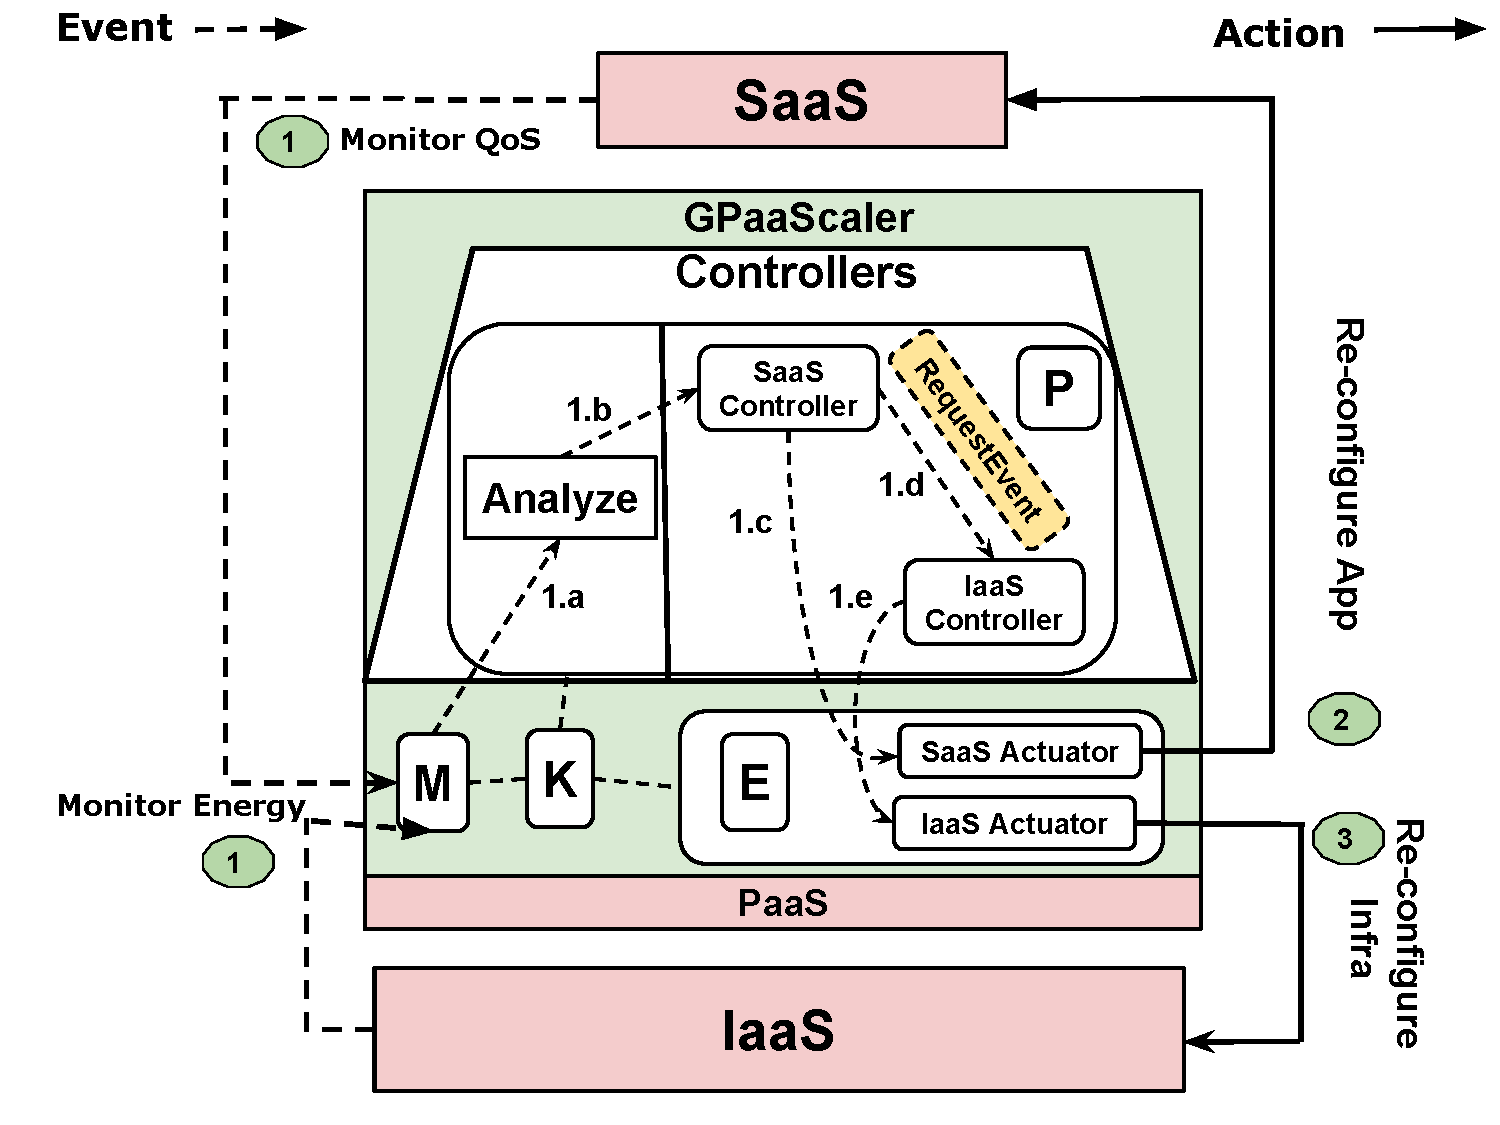
\includegraphics[scale=.35]{Graphs/test_gpaascaler.pdf}
\caption{GPaaScaler architecture}
\label{fig:GPaaScaler}
\end{figure}


